\subsection{Misure con TDC}

Collegando le uscite discriminate dei PMT 1 e 2 ai due ingressi dell'unico TDC funzionante%
\footnote{All'apparenza.}%
\,che abbiamo trovato in laboratorio, possiamo misurare i ritardi tra le risposte di due PMT posti uno di fronte all'altro sfruttando i fotoni dell'annichilazione. Per eseguire la misura usiamo come \emph{start} le coincidenze e ritardiamo i segnali dei due PMT, dato che lo start è successivo alla rivelazione dei fotoni. \`E stato scelto un ritardo di \SI{60}{ns} in modo che la differenza tra i tempi di arrivo $\Delta t=t_1-t_2$ possa essere sia positiva che negativa.

\marginpar{L'ultima frase non torna, sembra come se il fatto che sia \SI{60}{ns} sia particolarmente utile.
Che sia positiva che negativa dipendeva dal fatto che li avessimo ritardati.
Comunque la spiegazione è poco chiara per uno che non ha fatto le misure.}

Prima di eseguire la misura calibriamo il TDC con il generatore di funzioni usando come start un'onda quadra e come \emph{stop} lo stesso segnale ma ritardato in modo arbitrario.
Eseguiamo questa calibrazione per i due fondiscala disponibili: \SI{102}{ns} e \SI{510}{ns}.
Le calibrazioni hanno mostrato una buona linearità, ma la misura dei ritardi ha mostrato che il TDC, per un motivo a noi ignoto, non funziona.
\marginpar{In realtà a suo arbitrio può decidere di non funzionare anche quando lo testiamo con il generatore di segnali.}
Il grafico di Figura\autoref{100} è uguale a quello di Figura\autoref{500} nonostante le acquisizioni siano state fatte con due fondiscala diversi. Se nei due grafici ci fosse la stessa cosa, vedremmo la figura allargata di un fattore dato dal rapporto dei due fondiscala. Inoltre l'offset delle scale del TDC vale circa \SI{1}{digit}, quindi lo spostamento di circa \SI{50}{digit} del picco presente nei grafici non può essere spiegato da nessun effetto fisico.

\begin{figure}[h]
\centering
\subfloat
{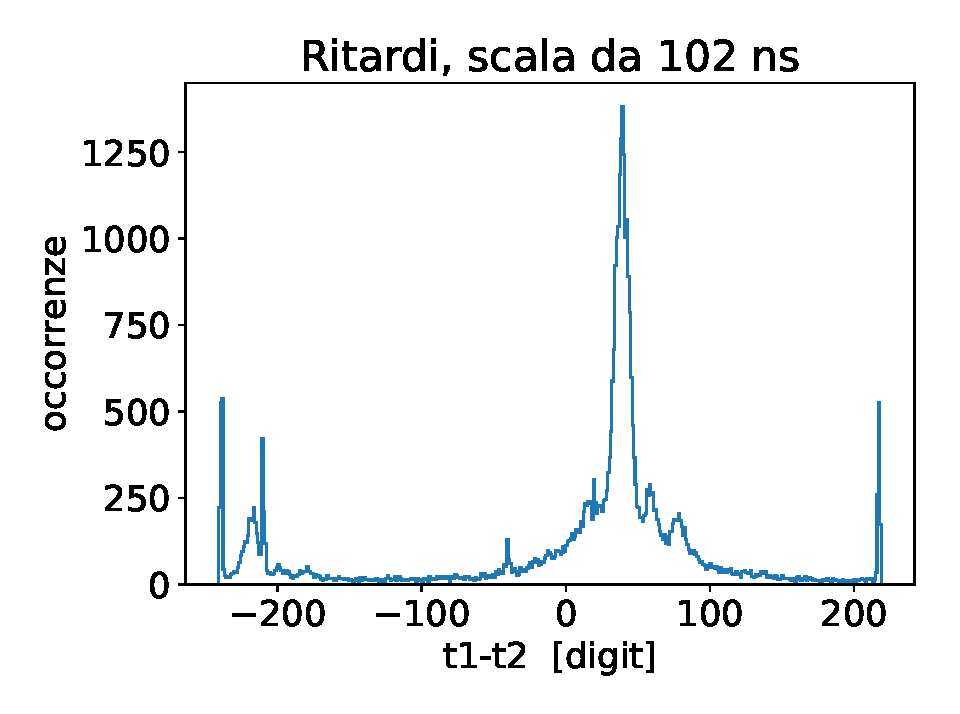
\includegraphics[width=17 em]{immagini/100}
\label{100}} \quad
\subfloat
{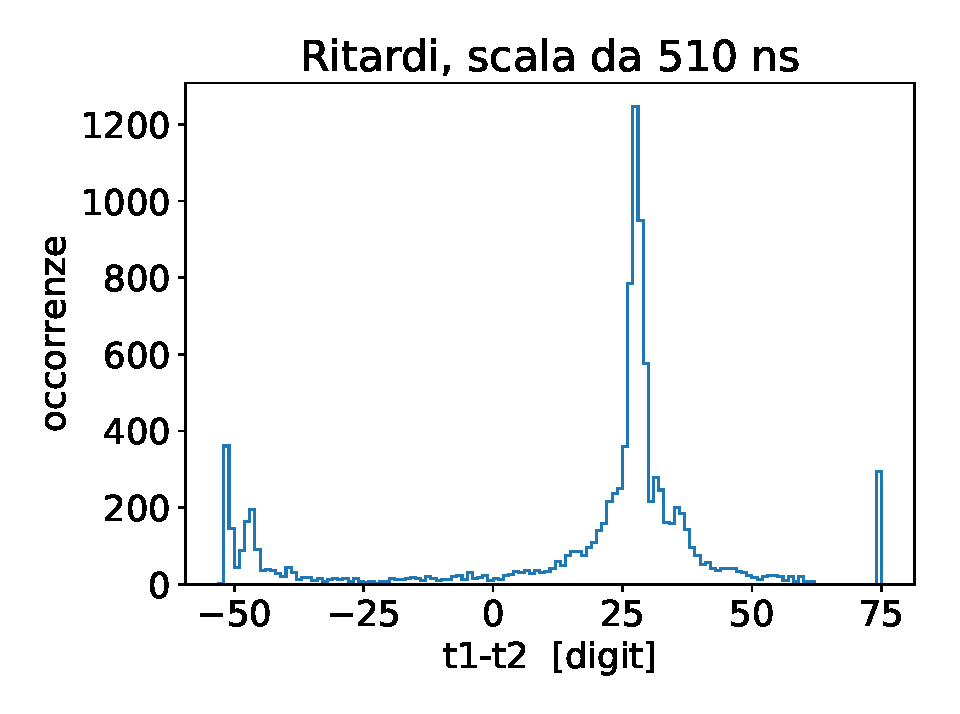
\includegraphics[width=17 em]{immagini/500}
\label{500}}

\caption{Misura di ritardo vista da entrambe le scale del TDC.}
\label{confronto}
\end{figure}

Questo problema ci impedisce di fare i facoltativi.